% first example chapter
% @author Jan Robert Rösler 
%
\chapter{Idee}

\section{DroNet ETH Zürich}
\note{Hier wird das DroNet Paper aufgegriffen und die draus entstandeene Idee erläutert}

Die ETH Zürich entwickelte 2018 eine eigene Architektur, mit dem Ziel durch Training auf Fahrbahnbildern eine Drone zu steuern. 
Das daraus entstandene, von Aufbau und Größe relativ einfach gehaltene Neuronale Netz, war der Anstoß für diese Arbeit. 

Kenn-Daten von DroNet (Berehcnungszeit, Parameter Layer)


Adaption auf das Carolo Cup Fahrzeug

Performance des Netzes in besimmten Metriken ist nicht intzeressant, da es um die Adaption auf Carolo Teststrecke geht.

Fahren auf der Strecke 

\note{Hervorhaben, welche Teile des DroNet Codes ich weiterverwede. Hard Mining, Auswertungsfunktionen, Architektur}

\section{Carolo-Cup}
aufgabenstellung beim carolocp
haus eigene strecke etc

\begin{figure}
	\centering
	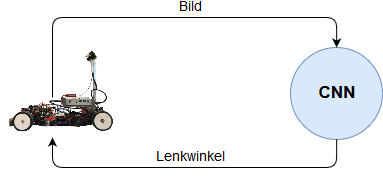
\includegraphics[scale=0.7]{figures/Aufbau.png}
	\caption{Eine tolle Grafik}
	\label{img:toll ist das}
\end{figure}

\section{Die Strecke}

\section{Das Fahrzeug}


\begin{figure}
	\centering
	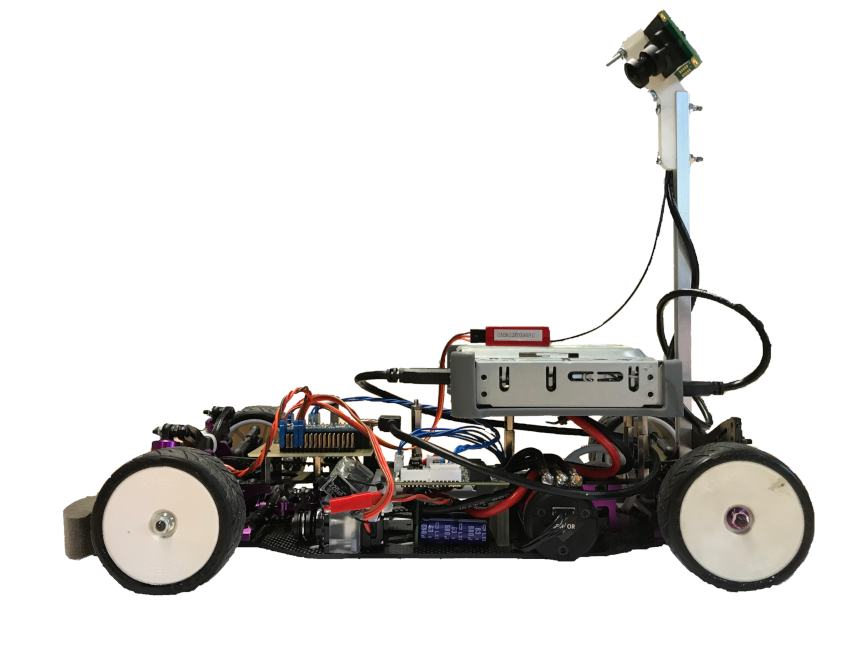
\includegraphics[scale=0.3]{figures/Fahrzeug.png}
	\caption{Das Carolo-Cup Fahrzeug}
	\label{img:Carolo-Fahrzeug}
\end{figure}
